\begin{figure}[H]
\centering
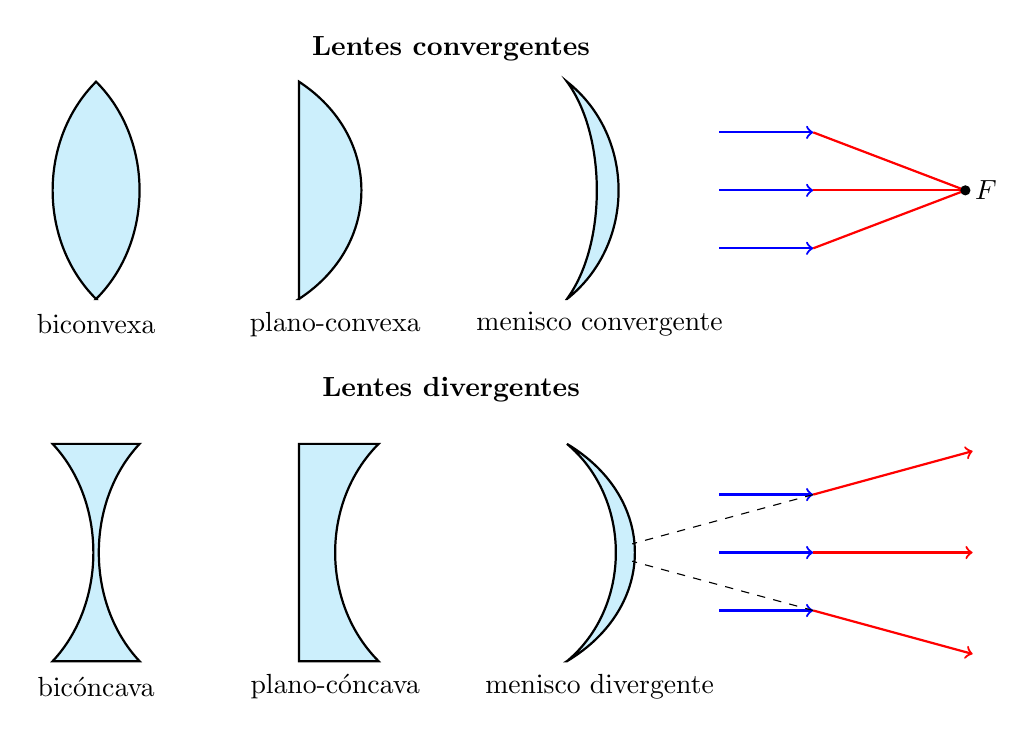
\begin{tikzpicture}[scale=0.92]
  \node[font=\bfseries] at (5.5,3.45) {Lentes convergentes};
  \node[font=\bfseries] at (5.5,-1.25) {Lentes divergentes};
  \filldraw[fill=cyan!20,thick] (0.6,0) .. controls (-0.2,0.8) and (-0.2,2.2) .. (0.6,3)
    .. controls (1.4,2.2) and (1.4,0.8) .. cycle;
  \node at (0.6,-0.35) {biconvexa};
  \filldraw[fill=cyan!20,thick] (3.4,0) -- (3.4,3)
    .. controls (4.55,2.25) and (4.55,0.75) .. cycle;
  \node at (3.9,-0.35) {plano-convexa};
  \filldraw[fill=cyan!20,thick] (7.1,0) .. controls (8.05,0.75) and (8.05,2.25) .. (7.1,3)
    .. controls (7.65,2.25) and (7.65,0.75) .. cycle;
  \node at (7.55,-0.35) {menisco convergente};
  \foreach \y in {0.7,1.5,2.3}{\draw[->,blue,thick] (9.2,\y) -- (10.5,\y);}
  \foreach \y in {0.7,1.5,2.3}{\draw[red,thick] (10.5,\y) -- (12.6,1.5);}
  \fill (12.6,1.5) circle (2pt) node[right] {$F$};
  \begin{scope}[yshift=-5cm]
    \filldraw[fill=cyan!20,thick] (0,0) .. controls (0.75,0.8) and (0.75,2.2) .. (0,3)
      -- (1.2,3) .. controls (0.45,2.2) and (0.45,0.8) .. (1.2,0) -- cycle;
    \node at (0.6,-0.35) {bicóncava};
    \filldraw[fill=cyan!20,thick] (3.4,0) -- (3.4,3) -- (4.5,3)
      .. controls (3.7,2.2) and (3.7,0.8) .. (4.5,0) -- cycle;
    \node at (3.9,-0.35) {plano-cóncava};
    \filldraw[fill=cyan!20,thick] (7.1,0) .. controls (8.0,0.75) and (8.0,2.25) .. (7.1,3)
      .. controls (8.35,2.25) and (8.35,0.75) .. cycle;
    \node at (7.55,-0.35) {menisco divergente};
    \foreach \y in {0.7,1.5,2.3}{\draw[->,blue,thick] (9.2,\y) -- (10.5,\y);}
    \draw[->,red,thick] (10.5,0.7) -- (12.7,0.1);
    \draw[->,red,thick] (10.5,1.5) -- (12.7,1.5);
    \draw[->,red,thick] (10.5,2.3) -- (12.7,2.9);
    \draw[dashed] (10.5,0.7) -- (8.0,1.38);
    \draw[dashed] (10.5,2.3) -- (8.0,1.62);
  \end{scope}
\end{tikzpicture}
\caption{Perfiles de lentes convergentes y divergentes y acción sobre rayos paralelos.}
\end{figure}